The geometry of the vessel with stenosis, as well as the initial position of the bolus, is schematically displayed in Figure \ref{fig:stenosis}. The vessel has raidus $R$ and length $L$. The stenosis is located at $A$ with width $S$ and remaining gap $G$. A bolus with width $W$ and the same radius as the vessel is placed at position $d$ at the initial time point. We further constrain these geometric parameters as follows
\begin{align}
    R&=L/20,\\
    d&=L/4,~W=L/20,\\
    A&=L/2,~S=L/10,~G=L/40.\\
\end{align}
\begin{figure}[htbp]
    \centering
    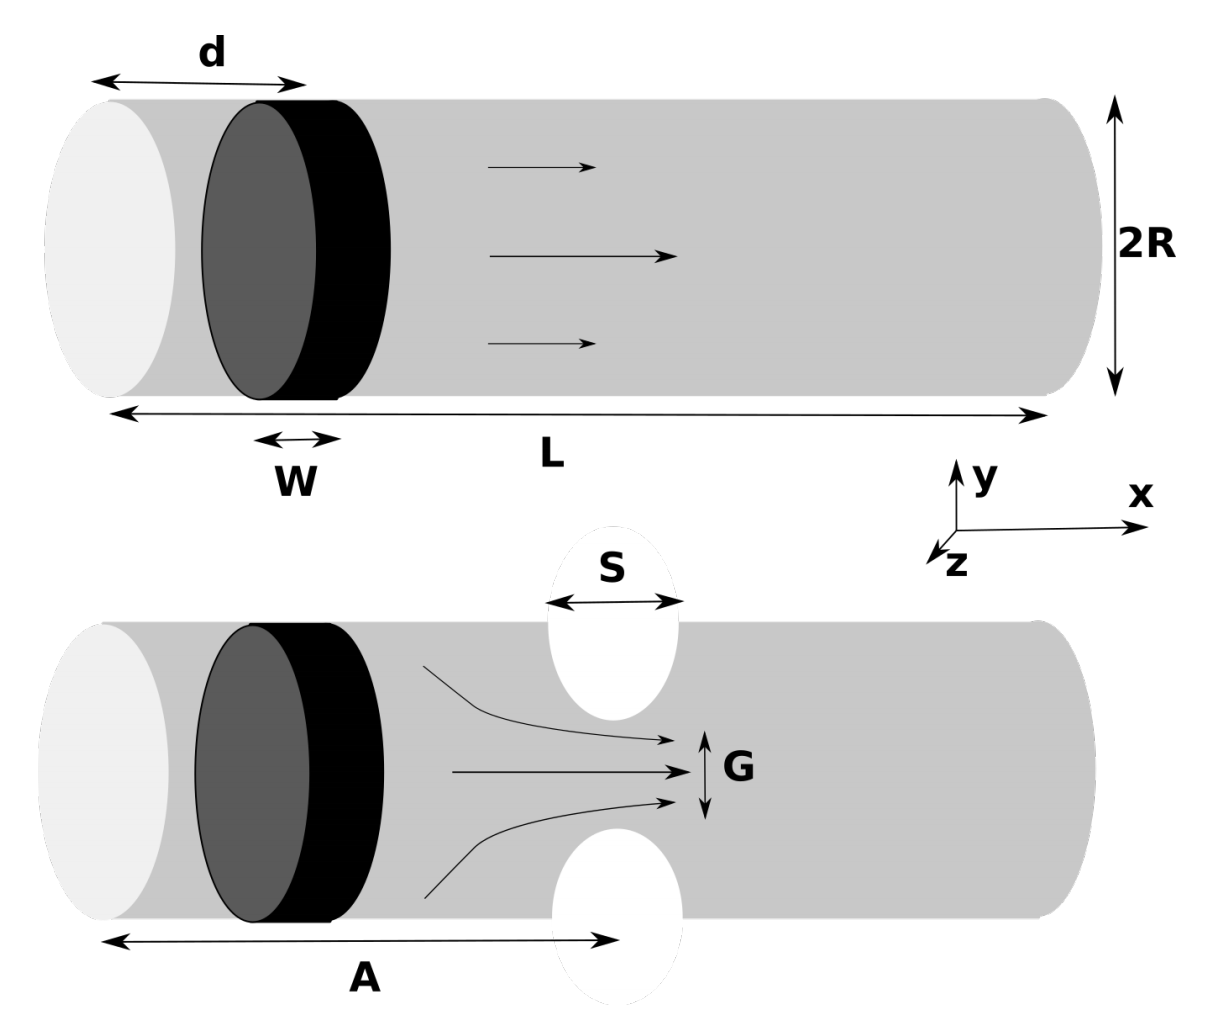
\includegraphics[width=0.6\textwidth]{YiqiXie/stenosis.png}
    \caption{Schematic setup of the problem.}
    \label{fig:stenosis}
\end{figure}

The blood vessel is treated as an impenetrable no-slip boundary. The left end of the vessel is the inlet applied with a driving blood flow
\begin{align}
    u_i(t)=\frac{\bar{u}}{2}\big(1+\cos(2\pi t/T)\big), 
\end{align}
where $T$ is the period of heartbeat. The right end is the outlet applied with fixed pressure (taken as 0 in the simulation). The initial drug concentration in the bolus is high as $c_0$. The boundary condition for the drug concentration is low as $c_1$ at both ends of the vessel. 

The values taken for the parameters are listed in Table \ref{tab:para_physprop}. The geometric scale of the system ($R$), as well as the drug diffusivity ($D$), is tuned to achieve different characteristic numbers, $Re$ and $Pe$. The relationships are
\begin{align}
    Re&=2\bar{u}R/\nu \\
    Pe&=\bar{u}R/D
\end{align}
The simulations are supposed to run through a total physical time of $4T$, with the first $1T$ used to stabilize the blood flow. However, because of the time limit of the project and possible errors from the HPC platform and the MUPHY code, some of the simulations are terminated before $4T$ is arrived. The detailed specifications of each simulation are listed in Table \ref{tab:sim_spec}.
\begin{table}[htbp]
    \centering
    \begin{tabular}{cc}
        \toprule
        Parameter & Value \\
        \midrule
        $\nu$ & 0.1 \\
        $\bar{u}$ & 0.01 \\
        $c_0$ & 1 \\
        $c_1$ & 0.01 \\
        $T$ & $10^6$ \\
        $R$ & (tuned) \\
        $D$ & (tuned) \\
        \bottomrule
    \end{tabular}
    \caption{Parameters of the physical system.}
    \label{tab:para_physprop}
\end{table}

\begin{table}[htbp]
    \centering
    \begin{tabular}{cc|cc|ccc}
        \toprule
         $Re$ & $Pe$ & $R$ & $D$ & Cores & Decomp. & Final Time Step \\
        \hline
         5  & 1.5 & 25 & 0.167 & 128 & $1\times1\times128$ & $4.0\times10^6$ \\
         5  & 3   & 25 & 0.083 & 128 & $1\times1\times128$ & $3.0\times10^6$ \\
         10 & 1.5 & 50 & 0.333 & 512 & $2\times2\times128$ & $1.3\times10^6$ \\
         10 & 3   & 50 & 0.167 & 512 &
         $2\times2\times128$ & $1.1\times10^6$ \\
        \bottomrule
    \end{tabular}
    \caption{Simulation specifications. }
    \label{tab:sim_spec}
\end{table}